%!TEX root = ../Lab_report.tex
%*******************************************************************************
%*********************************** Additional sections for analysis Chapter *****************************
%*******************************************************************************

\section{Electro-Osmotic flow}
Electro-Osmotic flow plays a crucial role in various scientific and industrial processes, especially in microfluidics, electrochemistry, and environmental science. In this work, the electro-osmotic flow of ions in a solution within a charged slit pore is investigated. We take a closer look at the density distribution of the ions as well as the flow profile of the solvent.
\subsection{System setup}
A snapshot of the system is shown in Figure \ref{fig:system1}. It consists of two infinite, parallel, charged walls with ions and a solvent in between. The ions are accelerated by a constant external electric field.  In order to reduce the degrees of freedom, the solvent is represented by an Lattice-Boltzmann Fluid. The wall charge is represented by 64 charged particles with the charge $q=\text{e}$ that are fixed on each wall. They create an electric field that is homogeneous enough for our application. To keep the system electrically neutral, 128 counter ions are placed between the walls. Periodic boundary conditions are used in the plane  parallel to the walls.  The electrostatic interactions are solved by the ELC algorithm. Additionally, all particles interact with each other and the walls via the Weeks-Chandler-Andersen potential. The simulation is performed with ESPResSo. A list of the system parameters can be found in the Appendix in Table \ref{tab:params}.
The python code can also be found in the Appendix. In the production run, the simulations is executed for 100000 integration steps and a step size $\Delta t= 0.01\,[t]$. Since the sampling of the flow and the density profile is numerically costly, only  every hundredth data point of the flow and the density profile was sampled.
\begin{figure}[H]
	\centering
	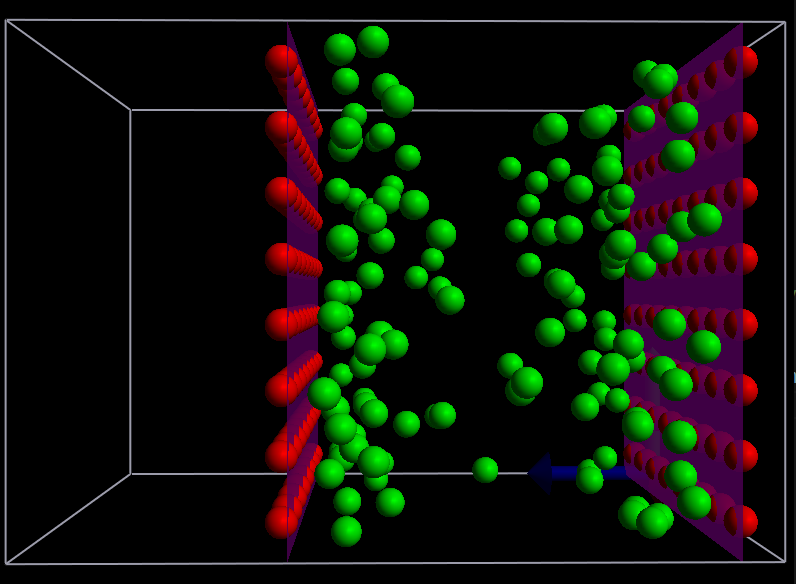
\includegraphics[width=\columnwidth]{Analysis_2/system}
	\captionsetup{width=\columnwidth}
	\caption{Visualization of the slit pore system. The wall charges (counter ions) are represented by red (green) spheres. The ELC gap is clearly visible on the left hand side of the left hand wall.}
	\label{fig:system1}
\end{figure}
\subsection{Results}
The flow profile of the solvent is a characteristic observable of a system with electro-osmotic flow. As explained in section \ref{ } it can be calculated analytically in the continuum limit. The analytical solution yields a characteristic flat flow profile. This profile is highest at the center and goes to zero at the boundary. Figure \ref{fig:slit_plot} shows the flow profile obtained by the simulation as well as the theoretical curve. It can be seen that there is a good agreement.

\begin{figure}[H]
	\centering
	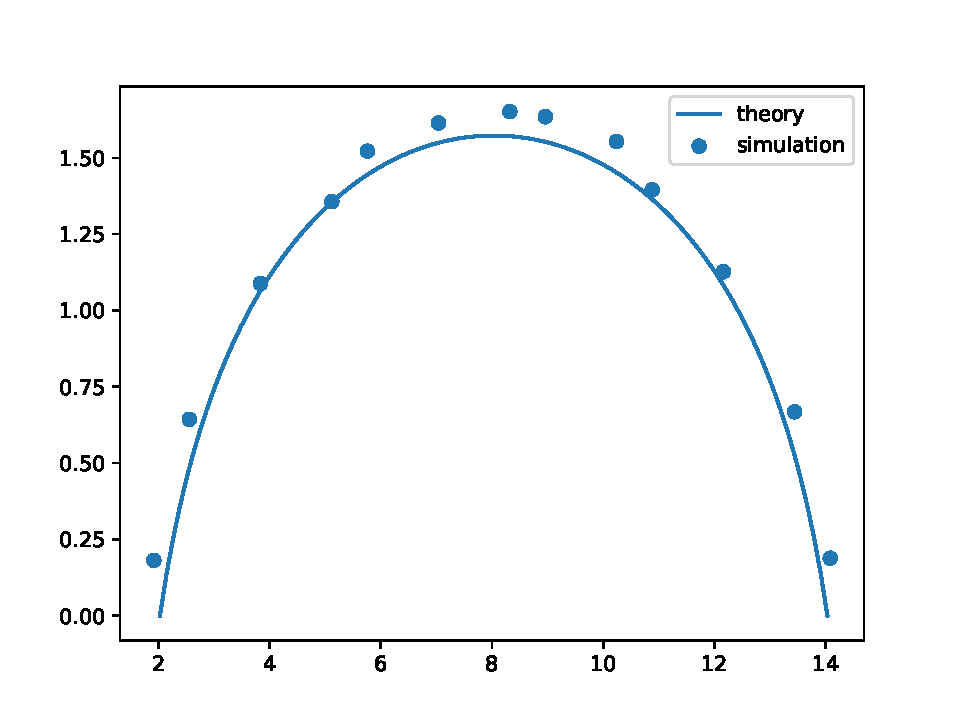
\includegraphics[width=\columnwidth]{slit_pore/prodrun_figs/fp}
	\captionsetup{width=\columnwidth}
	\caption{Comparison of the simulation data and the theoretical calculations of the flow profile.}
	\label{fig:slit_plot}
\end{figure}

Another interesting observable is the ion density profile. It can also be calculated analytically in the continuum limit. Due to the opposing charge of the wall and the ions, they attract each other. Therefore, the ions accumulate close to the boundary. Due to the repulsion between  the ions, not all of the ions condensate at the wall. This behavior can be seen in Figure \ref{fig:slit_plot2}. There is also an excellent agreement between the theoretical curve and the simulation data.
\begin{figure}[H]
	\centering
	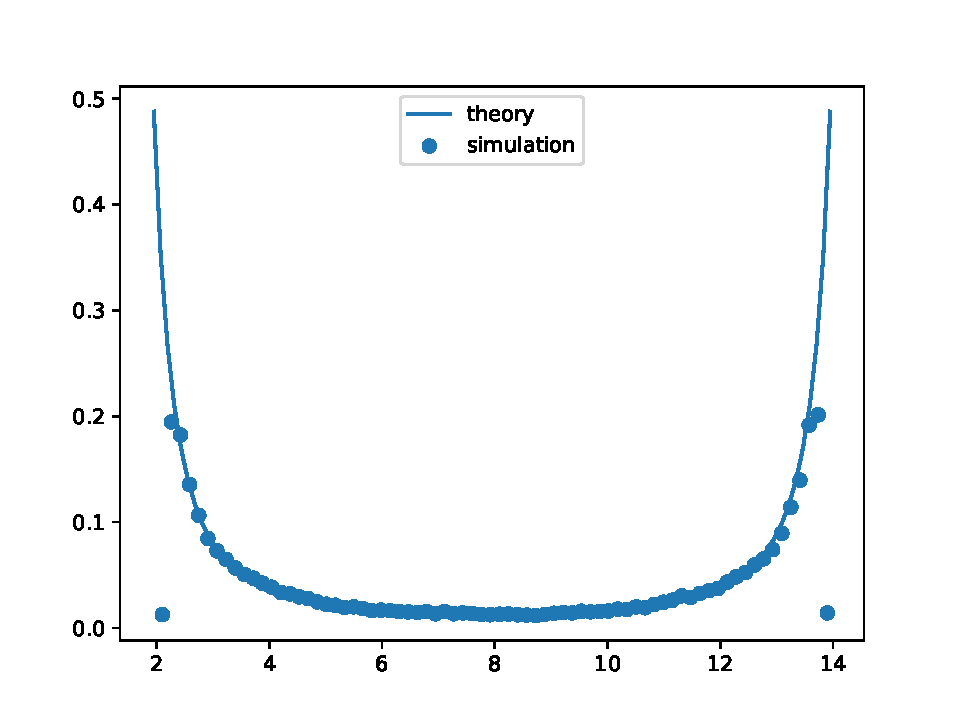
\includegraphics[width=\columnwidth]{slit_pore/prodrun_figs/id}
	\captionsetup{width=\columnwidth}
	\caption{Comparison of the simulation data and the theoretical calculations of the ion density.}
	\label{fig:slit_plot2}
\end{figure}
